\documentclass{report}

\usepackage[UTF8]{ctex}
\usepackage{listings}
\usepackage{xcolor}
\usepackage{graphicx}
\usepackage{float}

\lstset{
    numberstyle= \tiny, 
    keywordstyle= \color{red!100!green!90!blue!70},
    commentstyle= \color{red!50!green!50!blue!50}, 
    stringstyle= \color{red!20!green!80!blue!80},
    frame=shadowbox, % 阴影效果
    rulesepcolor= \color{ red!20!green!20!blue!20} ,
    escapeinside=``, % 英文分号中可写入中文
    xleftmargin=-5em,xrightmargin=-5em, aboveskip=1em,
    framexleftmargin=2em,
    language=python
} 


\begin{document}

\title{去中心化的聊天系统}
\date{}
\author{姓名:htx\\班级:18级计算机科学二班\\学号:18340057\\日期:2021.1.23}
\maketitle

\section*{一、 题目要求}
传统的聊天系统如微信等是一种中心化系统设计,数据集中存放。本项目的是设计一种去中心化的聊天系统,将聊天数据分散存储在各个客户端上。具体要求如下:
\begin{itemize}
\item 支持一对一聊天;
\item 支持聊天室群聊;
\item 能够满足实时性要求如响应时间控制在10ms以内;
\item 通信方式采用RPC;
\item 支持分布式系统一致性;
\item 具备一定的失效容错措施;
\item 需进行性能测试;
\item 聊天数据分散存储;
\end{itemize}


\section*{二、 解决思路}
首先,实现整个聊天系统的大前提是需要采用远程过程调用方法,因此不同于普通的聊天系统,发送消息由客户端将消息发送给服务器,接收消息由服务器将消息发给客户端,在我们的系统中,消息是不能由服务器主动向客户端发送的,而是需要客户端调用远程方法来进行消息的“拉取”。因此,考虑将客户端设计成两个线程并行运行,一个专门用于接收用户指令,另一个不断向服务器拉取消息,如果有新消息则在客户端显示。

其次,考虑到聊天数据是分布的,聊天记录应该保存在各个客户端,而服务器不会保存任何聊天记录。不同的客户端有着不同的聊天记录,在两个人的私聊或是群组聊天中,会有多份聊天记录保存在客户端中,这些记录应当是一致的。为了保持数据的一致性,必须用服务器来协调、整合客户端的聊天记录,并将整合好的记录返回给客户端用于本地保存,从而达成一致。也就是说,服务器需要具有缓存并整合聊天记录的能力,但不会实际保存聊天记录。客户端需要在合适的时候,比如发送消息时,将本地的聊天记录发送给服务器,让服务器进行多个客户端聊天记录的整合,再发回给各个客户端,从而达成数据的一致。

然而,为了满足系统的实时性特性,消息的整合需要进一步简化。如果每次双方聊天时都要将所有历史消息发给服务器,经整合后再发回客户端,会极大降低性能。在群聊中消息量更是庞大。因此,客户端只在打开私聊或者进入群聊时才把历史聊天记录推送给服务器。在私聊过程中,正常收发消息时,发送和收到的消息只写入客户端本地的聊天记录中,而不保存在服务器,服务器也不会对这些消息进行进一步的整合。而在群聊中,可能有多个用户陆陆续续地进入聊天室,每次有用户进入时都会推送它的本地聊天记录。如果要让其他用户重新推送一遍聊天记录进行整合也会降低性能,因此对于群聊,可以让服务器缓存群聊信息便于有用户推送本地聊天信息后进行快速整合。当所有用户从群聊退出后,群聊记录被保存在各个客户端,而服务器中的缓存信息被删除。这样可能会导致数据不一致的可能性增加,但在聊天系统的场景下,保护了更加重要的实时性。

这样一来,上述的一致性方法使得整个分布式系统也具备了一定的失效容错措施。考虑到在分布式聊天系统中,分布的是聊天数据,那么可能失效的节点应当是各个客户端。而客户端本身失效就不能进行正常聊天,因此只考虑客户端的聊天记录失效的问题。在某个客户端的聊天记录失效(如被删除或读取失败)后,通过上述的一致性实现原则,在私聊中对方上线后会将本地聊天记录推送给服务器,服务器再将记录发给客户端即可。群聊的过程也同理,只是群聊中有多个客户端的本地记录,这些本地记录被上传至服务器进行整合后,再发给失效节点即可。

总之,整个分布式聊天系统由一个服务器和多个客户端组成。客户端负责在本地保存聊天记录、向服务器推送本地聊天记录、向服务器发送私聊或群聊消息;服务器复杂接收各个客户端的记录,进行整合后发回各个客户端,并协调各个私聊和群聊的关系。针对题目要求的各个问题,都有了对应的解决方案:

\begin{itemize}
\item 支持一对一聊天:服务器进行聊天对象的协调
\item 支持聊天室群聊:服务器进行群聊的协调
\item 能够满足实时性要求:客户端发的消息立即被发给其他客户端
\item 通信方式采用RPC:客户端向服务器发送消息、拉取消息
\item 支持分布式系统一致性:服务器整合客户端的本地消息并发回客户端
\item 具备一定的失效容错措施:由一致性实现
\item 聊天数据分散存储:聊天数据冗余存储在各个客户端
\end{itemize}

\section*{三、 实现细节}
我使用的编程语言为python3,实现平台为windows。

\subsection*{3.1 RPC的实现}
为了实现RPC,我使用了python的rpyc库。在服务器包含如下库:
\begin{lstlisting}
from rpyc import Service
from rpyc.utils.server import ThreadedServer
\end{lstlisting}
在服务器声明一个服务类,在类中定义的函数如果以"exposed\_"开头,则能够被客户端调用,以客户端登录的函数为例:
\begin{lstlisting}
class ChatService(Service):
    # 客户端登录,服务器记录在线状态        
    def exposed_login(self, user_name):
        global client_num
        if user_name in client_name:
            return False
        else:
            client_num += 1
            client_name.add(user_name)
            print('连入用户:', user_name)
            return True
\end{lstlisting}
将类的定义送入相关函数,并创建线程进行RPC的管理即可:
\begin{lstlisting}
# 创建线程开启服务
rpcServer = ThreadedServer(ChatService, port=9999, auto_register=False)  
rpcServer.start()
\end{lstlisting}
在客户端,只需要包含rpyc库,并通过同名函数调用的方法,就能直接调用服务器的函数,如上述的login函数可以通过如下方式调用:
\begin{lstlisting}
conn = rpyc.connect('localhost',9999)
conn.root.login(user_name)
\end{lstlisting}
如此一来,就实现了RPC。之后的所有方法都是基于RPC的。

\subsection*{3.2 客户端到服务器的连接与消息的拉取}
在客户端启动时,需要与服务器取得连接。客户端提供一个用户名user\_name给服务器,服务器将记录下客户端的在线状态,并统计在线人数。如果存在相同用户名的用户则会要求客户端重新提供用户名。

客户端调用:
\begin{lstlisting}
login_status = conn.root.login(user_name)
\end{lstlisting}
服务器对应的RPC方法为:
\begin{lstlisting}
# 客户端登录,服务器记录在线状态        
def exposed_login(self, user_name):
    global client_num
    if user_name in client_name:    # 用户名重复则拒绝登录
        return False
    else:                           # 否则记录用户
        client_num += 1
        client_name.add(user_name)
        print('连入用户:', user_name)
        return True
\end{lstlisting}
同样在用户退出时需要对服务器进行断开,让服务器减少在线人数,并将用户从在线用户列表中去掉:
\begin{lstlisting}
# 用户注销
def exposed_logout(self, user_name):
    print('登出用户:', user_name)
    client_name.remove(user_name)
    global client_num
    client_num -= 1
\end{lstlisting}
在客户端连接服务器时,一方面可能需要向服务器发送消息,另一方面又可能随时从服务器收到消息。为了使用RPC方法,我们需要让客户端主动向服务器拉取消息。因此考虑使用双线程,一个线程专门用来向服务器拉取并打印消息,另一条线程为用户提供本地服务和发送用户消息。

拉取消息的线程采用同样的RPC接口创建:
\begin{lstlisting}
conn2 = rpyc.connect('localhost',9999)
t1 = threading.Thread(target = getMes, args = (conn2, user_name,))
t1.start()
\end{lstlisting}
其中,getMes函数为:
\begin{lstlisting}
# 第二个线程持续监听信道,返回新消息
def getMes(conn2, user_name):
    while 1:
        mes = None
        mes = conn2.root.getMes(user_name)
        if mes != None and mes != "":
            t, s, u, m = mes.split(' ', 3)
            # 在私聊状态下收到对方消息
            if status == 1 and user2 == u:
                appendMes(user_name, u, mes, True)
                mes2disp(mes)
            # 收到其他人的私聊消息
            elif status == 1:
                appendMes(user_name, u, mes, True)
                print('----提示:收到来自【'+u+'】的私聊消息----')
            # 收到群聊消息
            elif status == 2:
                appendMes(user_name, group, mes, False)
                mes2disp(mes)
\end{lstlisting}
客户端存在全局变量status用来记录当前的用户状态,为0表示没有进入任何聊天,为1表示正在私聊,有对应的全局变量user2表示聊天对象,为3表示正在群组聊天,有对应的全局变量group表示所在群组。当且仅当收到的消息来自私聊的对方时,可以直接打印消息,其余时候都只是提示收到了他人的消息而不会展示消息内容。需要建立私聊连接才能看到消息。其中,每条消息由四部分组成,每个部分之间由空格隔开。四个部分分别为:
\begin{itemize}
\item 时间戳,由time.time()获得,用于消息记录的排序
\item 消息状态,为1表示私聊消息,为2表示群聊消息
\item 消息的发送方,由用户名的字符串表示
\item 发送的消息本身(可以包含空格)
\end{itemize}
通过python的split功能可以对消息进行拆分,得到各个部分。通过调用mes2disp函数,可以将消息用用户名+消息内容的方式打印在屏幕上,方便查看:
\begin{lstlisting}
# 将记录转换成聊天消息并打印
def mes2disp(mes):
    if mes != "":
        t, s, u, m = mes.split(' ', 3)
        print('【'+u+'】'+ m)
\end{lstlisting}
在服务器端,存在一个字典message,将用户名映射到一个字符串。如果存在这样的映射,则表示该用户可以拉取对应的字符串作为消息,拉取后删除字符串防止重复拉取:
\begin{lstlisting}
# 接收消息
def exposed_getMes(self, user_name):
    if user_name not in message.keys():
        return ""
    else:
        mes =  message[user_name]
        del message[user_name]
        return mes
\end{lstlisting}


\subsection*{3.2 客户端的聊天记录保存机制}
每当客户端进入私聊或群聊时,就要读取保存在客户端本地的聊天记录。聊天记录保存在本地的chatting log文件夹下。如果是A本地的A与B私聊的记录,则记录名为A\_B.txt,若为A本地的B群的群聊记录,则记录名为A\_\_B.txt(两条下划线)。聊天记录的每条消息和上述一致,每条消息间用换行符隔开。函数参数的前两个为两个聊天用户(如果是群聊则第二个参数为群名),第三个参数表示是否为私聊,有True和False两种取值。
\begin{lstlisting}
# 读取本地聊天记录
def loadMes(user1, user2, private):
    if private:
        slt = '_'
    else:
        slt = '__'
    file_name = 'chatting log\\' + user1 + slt + user2 +'.txt'
    mes = ""
    # 打开本地聊天记录文件
    try:
        f = open(file_name, 'r')
        for eachLine in f:
            mes = mes + eachLine
        f.close()
    # 若不存在聊天记录则新建
    except:
        f = open(file_name, 'w')
        f.close()
    return mes
\end{lstlisting}
读取聊天记录后,客户端将向服务器推送聊天记录,由服务器整合多个客户端的聊天记录并返回一致化后的聊天记录。由私聊为例,客户端调用loadMes函数读取本地记录后发给服务器并接受返回的一致记录:
\begin{lstlisting}
old_mes = loadMes(user_name, user2, True)
res = conn.root.pushPrivateMes(old_mes, user_name, user2)
saveMes(user_name, user2, res, True)
\end{lstlisting}
得到返回结果后调用saveMes函数,用已经一致的聊天记录直接覆盖之前的聊天记录。在收到新消息时,调用appendMed函数直接在聊天记录中添加新增记录,而不需要重新向服务器发送消息进行整合,从而保证系统的实时性。

\subsection*{3.3 私聊的具体流程}
客户端进入私聊后,确定私聊的对象,并读取本地的聊天记录推送给服务器,服务器整合后发回本地进行保存:
\begin{lstlisting}
# 确立私聊对象
user2 = input('请输入私聊对象的用户名:')
if user_name == user2:
    print('不能建立与自己的私聊!')
    continue
# 拉取本地聊天记录并推送到服务器
old_mes = loadMes(user_name, user2, True)
res = conn.root.pushPrivateMes(old_mes, user_name, user2)
saveMes(user_name, user2, res, True)
status = 1
print('进入与', user2, '的私聊状态,输入exit退出私聊')
# 打印历史消息
mes = res.split('\n')
for each in mes:
    mes2disp(each)
\end{lstlisting}
服务器需要接收并整合不同客户端的聊天记录以维护一致性。客户端会维护一个字典private\_channel,由一个二元组映射到一条字符串。二元组(user1, user2)的映射结果表示user1本地的user1和user2私聊的聊天记录。如果同时存在(user1, user2)和(user2, user1)的记录缓存,则需要对二者进行整合。
\begin{lstlisting}
    # 收集、整合、推送私聊记录
    def exposed_pushPrivateMes(self, old_mes, user1, user2):
        res = ""
        # 将use1的本地聊天记录暂存在服务器
        if old_mes != "":
            private_channel[(user1, user2)] = old_mes
\end{lstlisting}
消息的整合类似于归并排序。两个客户端的本地消息已经按照时间顺序排序好,我们只需要依次取出两边最新的消息,将更早的排在前,更晚的排在后即可。相同的消息只保留一条,防止出现重复。由于每条消息都记录了时间戳,时间戳表示1970年至今的秒数,直接使用时间戳比较大小即可比较不同消息的先后关系。在消息整合后返回消息前,还要需要将服务器中缓存的消息记录删掉。最终服务器不保存任何聊天记录,所有记录都被保存在客户端本地。
\begin{lstlisting}
        # 整合消息
        if (user2, user1) in private_channel.keys():
        mes1 = old_mes.split('\n')
        mes2 = private_channel[(user2, user1)].split('\n')
        i = 0
        j = 0
        # 最后一行消息为空字符故要-1
        while i < len(mes1)-1 and j < len(mes2)-1:
            t1, m1 = mes1[i].split(' ', 1)
            t2, m2 = mes2[j].split(' ', 1)
            # 比较时间戳,较小的排在前
            t1 = float(t1)
            t2 = float(t2)
            if t1 > t2:
                res = res + mes2[j] + '\n'
                j += 1
            elif t1 < t2:
                res = res + mes1[i] + '\n'
                i += 1
            else:
                res = res + mes1[i] + '\n'
                i += 1
                j += 1
        while i < len(mes1)-1:
            res = res + mes1[i] + '\n'
            i+= 1
        while j < len(mes2)-1:
            res = res + mes2[j] + '\n'
            j+= 1
        # 删掉服务器的聊天记录缓存
        del private_channel[(user2, user1)]
    else:
        res = old_mes
    return res
\end{lstlisting}
客户端之后进入私聊状态,随时可以发送新的消息。输入消息后,先按照时间戳+消息状态+用户名+消息内容的格式进行封装,直接写入本地记录,再调用sendPrivateMes方法发给服务器,让服务器转发给对方。
\begin{lstlisting}
while 1:
    mes = input()
    # 退出私聊
    if mes == 'exit':
        status = 0
        user2 = None
        break
    else:
    # 消息 = 时间戳 + 状态 + 发送者 +发送内容
        print('【'+user_name+'】'+mes)
        mes = str(time.time()) + ' 1 ' + user_name + ' ' + mes +'\n'
        appendMes(user_name, user2, mes, True)# 写入本地聊天记录
        conn.root.sendPrivateMes(user_name, user2, mes)# 发给服务器
\end{lstlisting}
服务器只需要改动上述的消息字典即可让消息被对方拉取,从而收到消息:
\begin{lstlisting}
# 私聊消息处理
def exposed_sendPrivateMes(self, user1, user2, mes):
    message[user2] = mes
\end{lstlisting}
\subsection*{3.4 群聊的具体流程}
群聊的流程大体与私聊一致,只不过要加入群组成员的额外管理方案。

同样,在客户端输入群聊名称后读取本地聊天记录发给服务器,让服务器返回整合后的聊天记录后对本地记录进行重写并打印:
\begin{lstlisting}
    group = input('请输入群聊名称:')
    # 拉取本地聊天记录并推送到服务器
    old_mes = loadMes(user_name, group, False)
    res = conn.root.pushGroupMes(old_mes, user_name, group)
    saveMes(user_name, group, res, False)
    status = 2
    print('进入在', group, '的群聊状态,输入exit退出群聊')
    # 打印历史聊天记录
    mes = res.split('\n')
    for each in mes:
        mes2disp(each)
\end{lstlisting}
服务器需要管理各个群的群名,以及统计群下的所有成员。需要变量group\_num记录群的总数。字典group\_name将群名的字符串映射到该群中所有成员的集合中;字典group\_channel则记录该群的最终整合消息,初始化为空:
\begin{lstlisting}
    # 推送群聊记录
def exposed_pushGroupMes(self, old_mes, user, group):
    global group_num
    # 若群聊不存在则新建群聊
    if group not in group_name.keys():
        group_name[group] = set({})
        group_num += 1
        group_channel[group] = ""
    # 将当前用户加入群聊
    group_name[group].add(user)
    print(user, '加入群聊', group)
\end{lstlisting}
如同上述消息整合方法一样,每有一个用户将群聊记录推送到服务器,服务器就要对该群的聊天记录group\_channel[group]进行一轮整合并发回推送的客户端。代码基本相同,这里不再赘述。

需要注意的是,由于一个群组中可能有多个成员,每次有成员进入时就要求所有成员都重新发送消息进行整合会极大降低效率,因此服务器需要一直保存整合后的消息记录,以便新记录来到时能够快速整合。当所有群员退出群聊时,群聊记录在服务器中被删除。
\begin{lstlisting}
# 保存整合的消息
    group_channel[group] = res
    return res
\end{lstlisting}
同样,客户端可以随时发送消息给服务器让服务器将消息转发给其他成员。由于服务器维护了一个当前全部群员的集合,只需要将消息发给每个人即可。需要注意的是,有人发消息表示该群必然存在成员,因此群消息的缓存同时也必须更新:
\begin{lstlisting}
# 群聊消息处理
def exposed_sendGroupMes(self, group, mes):
    group_channel[group] += mes
    for each in group_name[group]:
        message[each] = mes
\end{lstlisting}
当用户退出群聊时,服务器也要更新当前的群员状态,删去成员:
\begin{lstlisting}
    # 退出群聊
    def exposed_exitGroup(self, user_name, group):
        print(user_name, '退出群聊', group)
        group_name[group].remove(user_name)
\end{lstlisting}
除了上述的功能外,我还设计了客户端通过RPC方法向服务器查询当前在线用户、当前已有群组的功能,实现较为简单,不在报告中赘述。
\section*{四、 结果展示}
\subsection*{4.1 私聊功能展示}
服务器不涉及人为交互,将服务器程序打开即可。

首先打开一个客户端,使用用户名"小A",目前除了小A没有任何人在线:

\begin{figure}[h]\centering
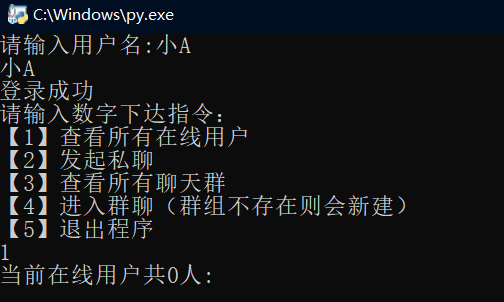
\includegraphics[scale=0.3]{pic/1.png}
\end{figure}
让小A向小B发送一条消息。注意,现在小A的聊天记录存在该消息,但小B的聊天记录不存在该消息。

\begin{figure}[h]\centering
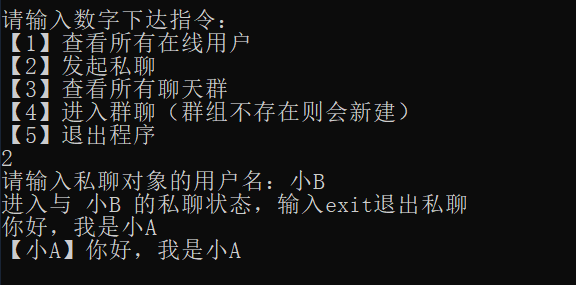
\includegraphics[scale=0.3]{pic/2.png}
\end{figure}
此时小B登录,拉取消息的线程可以发现新消息。小B查看在线用户,可以看到小A。

\begin{figure}[h]\centering
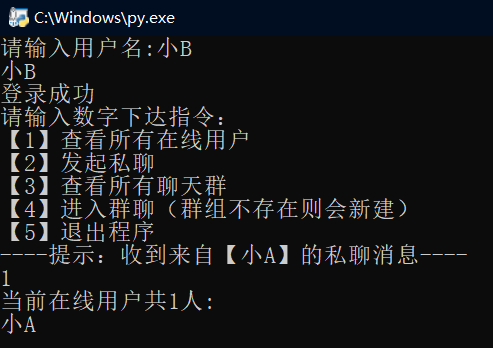
\includegraphics[scale=0.3]{pic/3.png}
\end{figure}
小B打开私聊连接时向服务器发送记录并拉取整合后的记录,可以看到消息记录出现了小A发送的消息,小B能够成功收到自己在线下时小A发的消息,二者的聊天记录达成了一致。

\begin{figure}[h]\centering
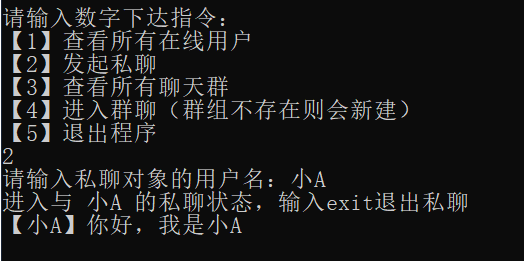
\includegraphics[scale=0.3]{pic/4.png}
\end{figure}
在线上发送消息可以直接进行本地消息记录的改写而不需要重新整合聊天记录。小B发送消息,小A可以马上收到:

\begin{figure}[h]\centering
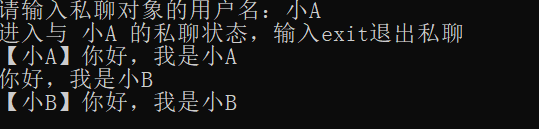
\includegraphics[scale=0.3]{pic/5.png}
\end{figure}
\begin{figure}[h]\centering
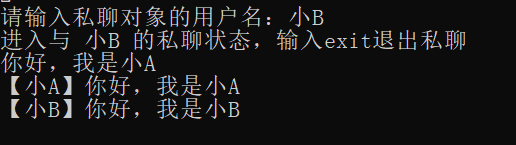
\includegraphics[scale=0.3]{pic/6.png}
\end{figure}
小A退出私聊后重新进入,也能正常地读取历史聊天记录:

\begin{figure}[H]\centering
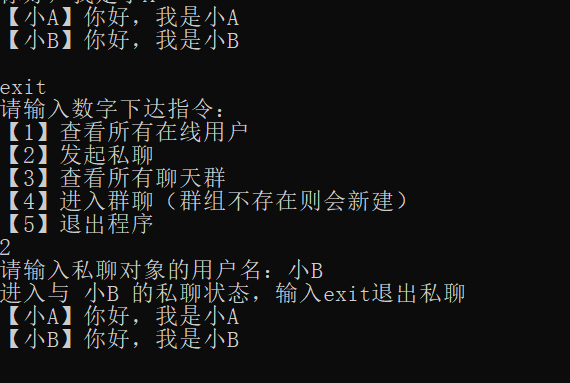
\includegraphics[scale=0.3]{pic/7.png}
\end{figure}
 
 \subsection*{4.2 群聊功能展示}
让小A和小B先在一个名为sysu的群聊中进行对话:

\begin{figure}[H]\centering
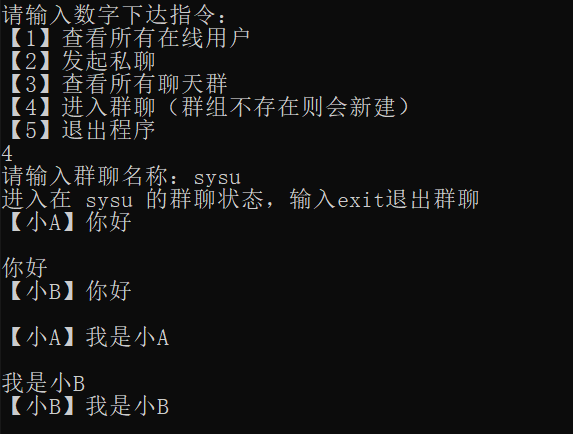
\includegraphics[scale=0.3]{pic/8.png}
\end{figure}
然后让小C登录,可以查看已有的群聊:

\begin{figure}[H]\centering
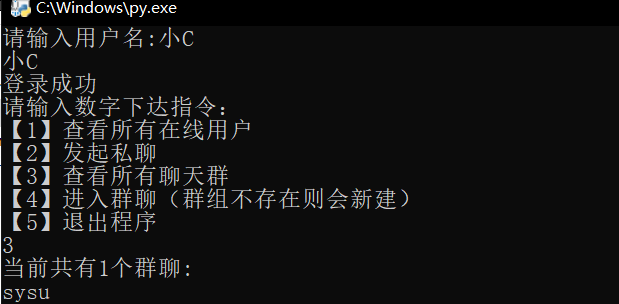
\includegraphics[scale=0.3]{pic/9.png}
\end{figure}
与私聊不同的是,在群聊中,因为小C并未加入sysu群组,因此不会拉取到任何聊天记录,也就是说,小C的本地没有sysu群的聊天记录,而且也不能从服务器拉取到聊天记录。然而在小C加入群聊时,向服务器推送本地消息,可以收到服务器发回的整合后的消息,从而得到完整的聊天记录,使得三人本地的聊天记录一致:

\begin{figure}[H]\centering
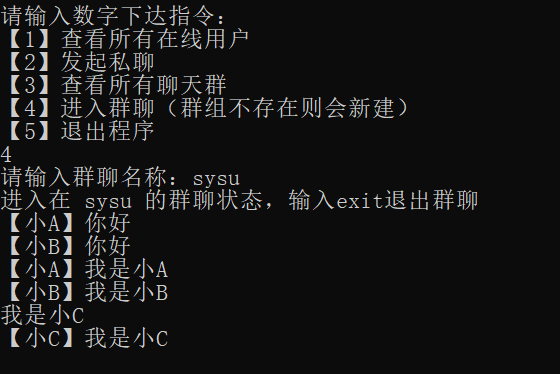
\includegraphics[scale=0.3]{pic/10.png}
\end{figure}

\subsection*{4.3 性能测试}
以私聊为例, 在接收消息的函数getMes()加上一句:
\begin{lstlisting}
    print('收到消息时间戳:', time.time())
\end{lstlisting}
并且将消息发送附上的时间戳打印出来,即在mes2disp函数中加上:
\begin{lstlisting}
    print('发送消息时间戳:',t)
\end{lstlisting}
发送消息时就能看到发送和接收的时间戳。让小A接收来自小B的三条信息:

\begin{figure}[H]\centering

\includegraphics[scale=0.3]{pic/11.png}
\end{figure}
“我是小A”和“我是小B”的两条信息来自之前私聊测试的历史记录。之后三条“来自小B的性能测试”是新发送的消息。新消息的发送和接收的时间戳都被打印出来,时间戳以秒为单位,因此三条消息的发送延迟只有约5ms、3ms、3ms,小于要求的10ms。

在我的消息同步机制中,只有用户建立起私聊连接和进入群聊时才会进行本地聊天记录的一致化,此时聊天还未正式开始,因此性能损耗可以忽略。换句话说,消息的一致性不在聊天时维护,聊天时每次只是单条消息的收发,性能损耗极低,保证了在聊天应用场景下的实时性。

\section*{五、 遇到的问题}
在本次项目的实现过程中,我遇到的第一个问题就是RPC的使用问题。RPC强调的是客户端对服务器功能的调用,换句话说就是客户端存在需求时,对远程服务器的过程的主动调用。而在传统意义上的聊天系统中,服务器和客户端在消息收发的层面上来说应该是对等的。当客户端需要发送消息时,则直接发给服务器,而服务器需要发消息给客户端时,也是直接发给客户端。而在RPC的前提下,服务器不能“主动”地向客户端推送消息,而是需要等待被客户端调用。一开始我尝试的是让客户端的用户手动输入指令,向服务器拉取消息的方式,但后来发现这样极大降低的收发消息的效率,完全无法保证实时性要求。因此,最终我采用的设计是在客户端使用额外的线程持续向服务器拉取消息,在不影响用户发送消息的同时,又能及时地接受最新的消息。

其次是python的rpyc库的使用问题。服务器需要同时服务多个客户端,因此服务器必须也是多线程的。同时,考虑到服务器必须对用户和群组进行管理,多个线程肯定需要进行信息的交换。一开始,我误以为不同的线程共享的是同一个服务器类对象的实例,因此将当前在线人数、服务器的消息缓存等信息作为服务器类的成员变量进行管理,结果不能成功地收发消息和查看在线用户。经过调试和输出我发现,每个线程独立拥有一个服务器类的实例。因此我最终采用了共享全局变量来实现这些线程之间的通信,让消息能够正常传递和记录。

再者是消息一致性的维护问题。在我设计的系统中,消息记录都保存在客户端本地,同步时需要客户端将消息发送给服务器,服务器将这些消息整合后再发回各个客户端。如此一来,各个客户端的本地消息就能保持一致。但是同步的时机和机制还值得进一步考虑。一开始我的设计是,每次客户端本地消息更新时就马上推送到服务器,服务器进行整合后返回给全部需要保存该消息的客户端。如果是私聊且历史消息量不大的情况下,该机制基本没有什么问题。然而在群组通信中就会产生很严重的性能损耗。如果一个群组已经有了很多用户进行聊天,此时又有新用户加入时,服务器会要求全部的用户将自己本地的记录推送到服务器,进行整合后再发回各个客户端,这样一来,整个系统的实时性会变得极差。在考虑和权衡后,我决定,只在用户进入私聊或群聊时才进行消息同步,而且只对进入的那一个用户进行同步,在聊天过程中只是正常的收发消息,由各个客户端自己写入聊天记录而并不同步。这样一来,以一定的一致性为代价,有效地保障了实时性。

\section*{六、 总结}
 本次作业我实现了一个简单的分布式聊天系统,消息记录保存在各个客户端本地,而服务器不保存任何聊天信息,客户端与服务器的通信采用RPC方式。就最终效果来看,客户端之间能够正常地进行聊天,性能较好,而且聊天记录能够适时地同步,保证冗余信息的一致性。最重要的是,作为一个分布式系统,在满足信息分布式存储的前提下,整个系统较好地做到了功能的透明化。就使用来说,与传统的中心化聊天系统并没有什么差别,整个信息的分布与同步被较好地通过内在机制被屏蔽了,而分布式系统相较于传统的中心化系统,又调动了多台机器的运算与存储,潜在地提高了整个系统的规模可拓展性。
 
通过本次作业,我更进一步地了解了分布式系统的机制和实际应用方式,通过自己亲手实现,对数据的分布与同步又了更深的见解,同时也提高了自己对分布式项目的设计与实现能力。
\end{document}